\section{Fault Detection}

Fault detection deals with detecting system discrepancies, abnormal behaviour. It is the first step towards handling faults. It doesn't necessarily identify the source of the fault, just establishes the fact that a fault has occurred in the system. In redundant systems, fault handling can be achieved shutting down the actuator affected by the fault and reassining the tasks of the shut down actuator.


\subsection{Motor fault detection}

\subsubsection{Model Free Fault Detection}
\label{sec:ModelFreeFD}

Some faults can cause anomalies in signals that are easy to notice by simply analyzing the signal shape they produce. Discontinuities for example often hint at a fault. Since most signals are sampled discretely, discontinuities appear as large signal gradients. For example, if the angular velocity sensor in the reaction wheel motors fall to zero instantaneously, there's a good chance that a sensor fault has just occurred. Detecting faults through such anomalies require no knowledge of the system dynamics, thus they can be deemed as model free fault detection. \todo{add figure showing angular velocity signal dropping to zero and discrete time gradients in same graph + threshold level}

A reconfiguration scheme using anomaly detection in angular velocity sensors has been implemented in the simulation. The detection checks the magnitude of the angular velocity gradient, and if it's above the threshold, the fault detector module sends a fault signal to the reaction wheel supervisor system, which can decide to reconfigure the reaction wheel torque distribution. The signal equation is given by equation \ref{eq:modelFreeDetect}, where $\dot{\omega}_{thresh}$ denotes the treshold for fault signal generation, $\delta t$ denotes the sampling time.  $\dot{\omega}_{thresh}$ can be set according to maximum reaction wheel torque, maximum reaction wheel angular velocity and wheel friction. $\dot{\omega}_{thresh}$ should at  least be $\dot{\omega}_{thresh} > \frac{b \omega_{max} + \tau_{max}}{J_{motor}}$ if false fault signals are to be avoided.

\begin{equation}
\label{eq:modelFreeDetect}
FaultSignal_i = |\omega_{w,i}(k) - \omega_{w,i}(k-1)| > \dot{\omega}_{thresh} \Delta t
\end{equation}

\section{Motors fault detection}

\label{sec:structural}
\subsection{Structural Analysis}
Structural analysis studies the interrelation between parameters and variables of the system using constraints between them. It distinguishes known and unknown variables, according to whether they can be measured in the system or not. Then the unknown variables are expressed using the known ones according to the constraints. Structural analysis based residual signal require that unknown variables can be expressed redundantly. One of the constraints is used to express the unknown, the other to verify it. If there's a mismatch between the two, a fault is detected.

In case of fault detection in sensors, one constraint is between the measured and the actual values of a variable. In case of a sensor fault, there can be a considerable difference between the measured and the actual value of a variable.

Assumes that only one fault occurs at any given time, so faults cannot mutually neutralize each other. 

The constraints being used to detect faults in the motor are:

\ref{sec:motor} \todo{reference motor section properly}


\begin{equation}
V_a = R_a * i + k_e \omega
\end{equation}

$L_a$ is negligible

\begin{equation}
 k_{t}i  =J\dfrac{d\omega}{dt} + b\omega
\end{equation}

\begin{equation}
\tau = k_t i
\end{equation}

$d_1(\omega, \dot{\omega})$


\subsection{Alternative method for identifying reaction wheel fault}

With enough computational power the faulty reaction wheel can be detected through the calculated reaction wheel output torque, assuming only one reaction wheel is faulty. It is done by calculating the difference between 3D torque demand and actual 3D torque output. 

\begin{equation}
\vec{N}_{rw} = \underline{I}_s \dot{\vec{\omega}}  + \vec{\omega} \times \vec{h_{rw}} - \vec{N_{mt}} - \vec{N_{dist}}
\end{equation}

Then the difference between torque demand and torque output is calculated. The reaction wheel that has the most similar axis orientation to the torque difference is deemed as faulty.

\begin{equation}
\vec{N}_{rw}^{demand} - \vec{N}_{rw}^{actual} = 
\vec{N}_{rw}^{diff}
\end{equation}

\begin{equation}
 \pm \vec{N}_{rw}^{diff}  \stackrel{?}{\approx} \vec{axis} 
\end{equation}


\todo{mention unit vector notation, decide notation for axis, express axis according to q}

Note: the lag for torque change and wheel saturation has to be taken into account separately, as those don't count as faults. 
Thresholds should be applied.

\section{Magneto torquers  fault detection}

\subsection{Unknown Input Observer (UIO)}

Uncertainties and modeling errors may cause discrepancies between the actual system and the descriptor mathematical model. Linearization and simplifications which make the system more manageable may lead also to uncertainties. All these uncertainties can have an effect on the system dynamic behavior through the input signals.   
A residual, fault indicator, based on observer design can be robust regarding the unknown input signals by making the effect of unknown inputs(UI) insensitive to the residual and thus making possible to maximize the detectability of a fault. 
Following \cite{UIO}     

\section{Magnetorquers  fault detection}
For magnetorquers fault detection, two types of structural analysis were implemented. First, a locally structure analysis for each magnetorquer was implemented, and second a second a structure analysis using the satellite dynamics.
\subsection{Magnetorquers local structural analysis} \label{sec: MTStructAnal}
Using the Biot-Savar law from \ref{eq:BS}, the residual for the magnetorquer is generated using the following equation:
\begin{flalign}
	residual = B - \frac{4 \mu_0}{\sqrt{2} \pi L} I
	\label{eq:BfS}
\end{flalign} 
where \\
$\vec B$ is the magnetic field \\
$\mu_0$ is a constant called permeability of free space \\
$I$ is the current \\
$L$ is the length of the coil

In equation \ref{eq:BfS} the magnetic field is measured and based on this measurement the magnetic moment can be deducted, but for the residual is not necessary, because if it is correct then the magnetic moment should be as expected using magnetic sensors for checking, unless the shape of the coil changes, perhaps due to some physical movement of the system.

\subsection{Unknown Input Observer (UIO)} \label{sec:UIO}
Uncertainties and modeling errors may cause discrepancies between the actual system and the descriptor mathematical model. Linearization and simplifications which make the system more manageable may lead also to uncertainties. All these\nomenclature[A]{\textbf{UIO}}{Unknown Input Observer } uncertainties can have an effect on the system dynamic behavior through the input signals.   
A residual, fault indicator, based on observer design can be robust regarding the unknown input signals by making the effect of unknown inputs(UI) insensitive to the residual and thus making possible to maximize the detectability of a fault. The dynamic equation of the system can be written as 
\nomenclature[A]{\textbf{UI}}{Unknown Input}
%

\begin{equation}
\dot{\vec{x}} = \underline A\vec{x}+\underline B \vec{u}+\underline E\vec{d}
\label{stateObs}
\end{equation}
\begin{equation}
\vec{y} = \underline C \vec{x}
\end{equation}
%
where $\underline A$ ,$\underline B$ and $ \underline C $ are the system matrix, input and output matrix respectively and $\underline E$ is the distribution matrix of the unknown input or disturbance vector $\vec{d}$. Furthermore, $\vec{x}$ is the state vector $\vec{u}$ is the input vector and $\vec{y}$ is the output vector. The time dependency of the variables has been suppressed in order to relax the notation. Following \cite{UIO}, 
%
%
\\
\textit{An observer is defined as Unknown Input Observer for a system described by \eqref{stateObs} if the state estimation error vector $e$ approaches zero asymptotically regardless of the presence of the unknown input }
\\
The full order observer
\begin{equation}
\dot{\vec{z}} = \underline F\vec{z}+\underline{TB} \vec{u}+\underline K\vec{y}
\label{stateObs1}
\end{equation}
\begin{equation}
\hat{\vec{x}} = \vec{z} + \underline H \vec{x}
\end{equation}
with $\hat{\vec{x}}$ be the state estimate and $\vec{z}$ the state of the observer. When \eqref{stateObs1} is an observer for the system given by \eqref{stateObs} the dynamics of the errors vector($\vec{e} = \vec{x} - \hat{\vec{x}}$) can be written as\cite{UIO} 
%
\begin{equation*}
\dot{\vec{e}}= (\underline A-\underline H \underline C \underline A-\underline K1 \underline C)\vec{e} + (\underline A-\underline H \underline C \underline A-\underline K1 \underline C - \underline F)\vec{z}+ ((\underline A-\underline H \underline C \underline A-\underline K1 \underline C )\underline H-\underline K2)\vec{y}
\label{errordynamics}
\end{equation*}
\begin{equation*}
+ (\underline I - \underline {HC} - \underline T)\underline B\vec{u}	+(\underline I -\underline H\underline C)\underline E \vec{d}
\label{errordynamics45}
\end{equation*}
in the above equation the utility of $\vec{x}  = \vec{e} + \hat{\vec{x}} = \vec{e} + \underline H\vec{y}+\vec{z}$ is used. The estimation error may converge to zero if the following conditions hold true:
%
\begin{equation}
\underline F = \underline A-\underline H \underline C \underline A-\underline K1 \underline C
\label{errordynamics3}
\end{equation}
\begin{equation}
(\underline I - \underline{HC})\underline E = 0
\label{errordynamics4}
\end{equation}
\begin{equation}
\underline T = (\underline I - \underline H\underline C)
\label{errordynamics5}
\end{equation}
\begin{equation}
\underline K = \underline K_{1} +\underline K_{2}
\label{errordynamics6}
\end{equation}
\begin{equation}
\underline K_{2} =\underline F \underline H 
\label{errordynamics7}
\end{equation}
where $\underline K_{1}$ is designed freely by pole placement to give desired eigenvalues of the observer. The error dynamics if the \ref{errordynamics4}...\ref{errordynamics7} hold true can now be written as 
\begin{equation}
\dot{\vec{e}} = \underline F \vec{e}
\label{errordynamics8}
\end{equation}
consequently if the eigenvalues of $\underline F$ are to the left half plane, the error converges exponentially asymptotically to zero. 

A solution to \eqref{errordynamics4} is given by making use of the Moore-Penrose pseudo-inverse as
\begin{equation}
\underline H = \underline E (\underline{CE})^\dagger
\label{errordynamics9}
\end{equation}
with $(\underline{CE})^{+} = [(\underline{CE})^{T} (\underline{CE})]^{-1}\underline{CE})^{T} $.
A sufficient and rather necessary conditions for the UIO existence is the number of independent unknown inputs can not be larger than the number of independent measurements which leads to
\begin{equation}
rank (\underline{CE}) =rank( \underline E) 
\label{errordynamics10}
\end{equation}
and by denoting $\underline A1 = \underline A - \underline{HCA} $ that the pair $(\underline {CA1})$ is detectable and thus $F$ can have stable roots.
\subsubsection{Residual Generation}
The residual is used for fault detection and isolation thus should be decoupled from the unknown inputs(disturbances). The residual can be written as
\begin{equation*}
\vec{r} = \vec{y} - \underline C \hat{\vec{x}} 
\label{errordynamics11}
\end{equation*}
\begin{equation*}
= \vec{y} - \underline C (\vec{z} + \underline{H} \vec{y} ) 
\label{errordynamics12}
\end{equation*}
\begin{equation*}
= (\underline I  -\underline{ CH})\vec{y}   -\underline C \vec{z} 
\label{errordynamics13}
\end{equation*}
which is clear that does not depend on the disturbance vector. A simple threshold can be applied such that for the faulty case, if the magnitude of the residual is larger than the threshold then a fault has been occurred as
$\{\lVert \vec{r}\rVert \geq threshold \}$ else if $\{\lVert \vec{r}\rVert < threshold \}$ then the system is fault free. In the \figref{fig:residualobs} the block diagram of the nominal system and the observer can be seen along with the residual generator
\begin{figure}[H]
	\centering
	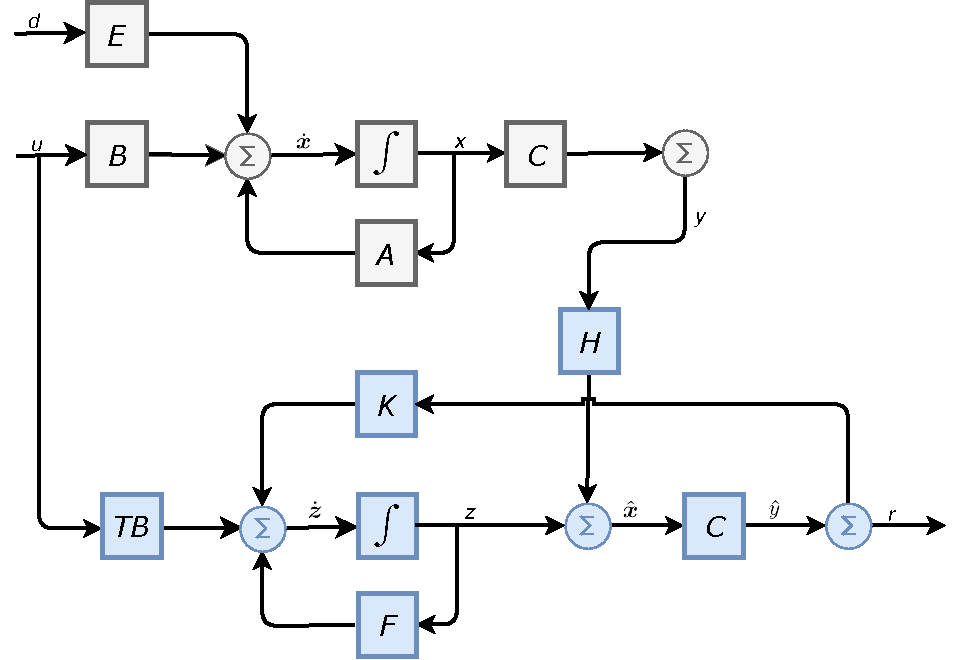
\includegraphics[width=0.7\linewidth]{figures/UIO}
	\caption{Observer based residual generator}
	\label{fig:residualobs}
\end{figure}
Moreover, in the \figref{fig:residualobstest} it can be seen how the state error converge asymptotically to zero from the initial conditions along with a change in the attitude of the satellite after 70 seconds.
\begin{figure}[H]
	\centering
	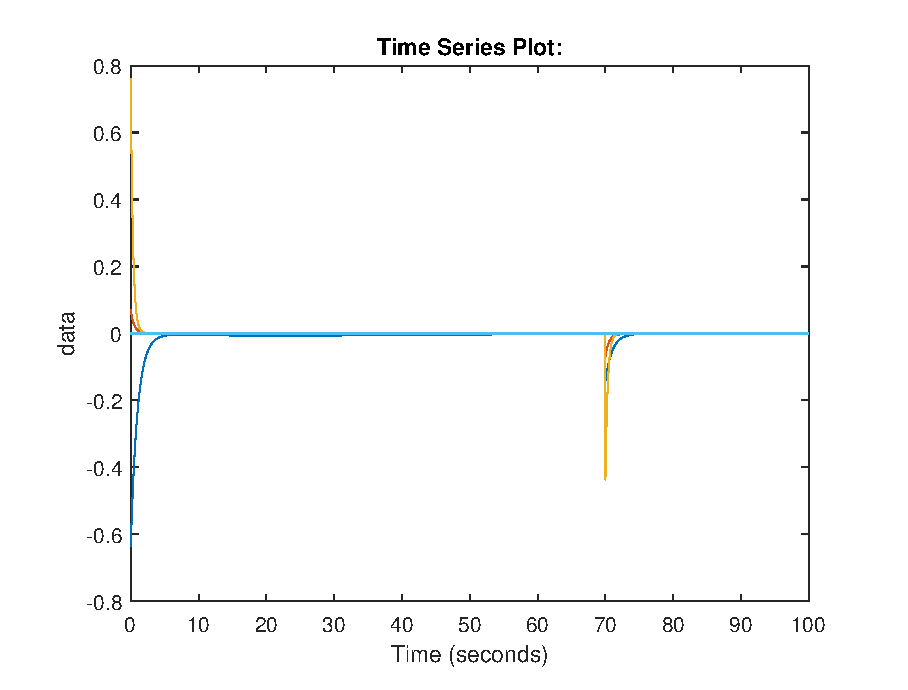
\includegraphics[width=0.7\linewidth]{figures/obstest}
	\caption{Convergence of the state estimation error to zero with the disturbance been decoupled}
	\label{fig:residualobstest}
\end{figure}
 Fault isolation is possible assuming that all the sensors are fault free. A descriptor model of the overall system with actuator fault can be written as \eqref{stateObs} by adding the actuator fault indicator in the equation as 
\begin{equation}
\dot{\vec{x}} = \underline A\vec{x}+\underline B \vec{u}+\underline E\vec{d} + \underline B\vec{f_{act}}
\label{stateObs34}
\end{equation}
where $\vec{f_{act}}$ represents the actuator faults. After the detection, faults can be isolated by deleting the $i_{th}$ column of the matrix B namely $\vec{b_{i}}$ and incorporating this along with the disturbance distribution matrix as
\begin{equation*}
E^{i} = [ E  \vec{b_{i}}]
\label{errordynamics14}
\end{equation*}
and furthermore, the $i_{th}$ component of the input vector $u_{i}$ is incorporated to the disturbance vector as 
\begin{flalign*}
\begin{bmatrix}
\vec{d} \\ u_{i}+f^{i}_{act}
\end{bmatrix}
\end{flalign*} 
leading to a bank of observers with each residual actuated by 2 inputs(without $i_{th}$) and all outputs. The detection of the fault is made by applying a threshold as  $\{\lVert r^{i}\rVert < Thr^{i} \}$ else if $\{\lVert r^{k}\rVert \geq Thr^{k} \}$ with $k = 1,...i-1,..i+1,5..r$.
%\subsection{CUSUM algorithm and change detection} 
%The evaluation of the residual which determines if the %actuator is faulty or fault free is based on the %cumulative sum (CUSUM), a sequential hypothesis %testing technique to detect changes on the noisy %signal. By changes are accounted changes on the mean %of the original signal. 



% \begin{figure}[H]
%	\centering
% 	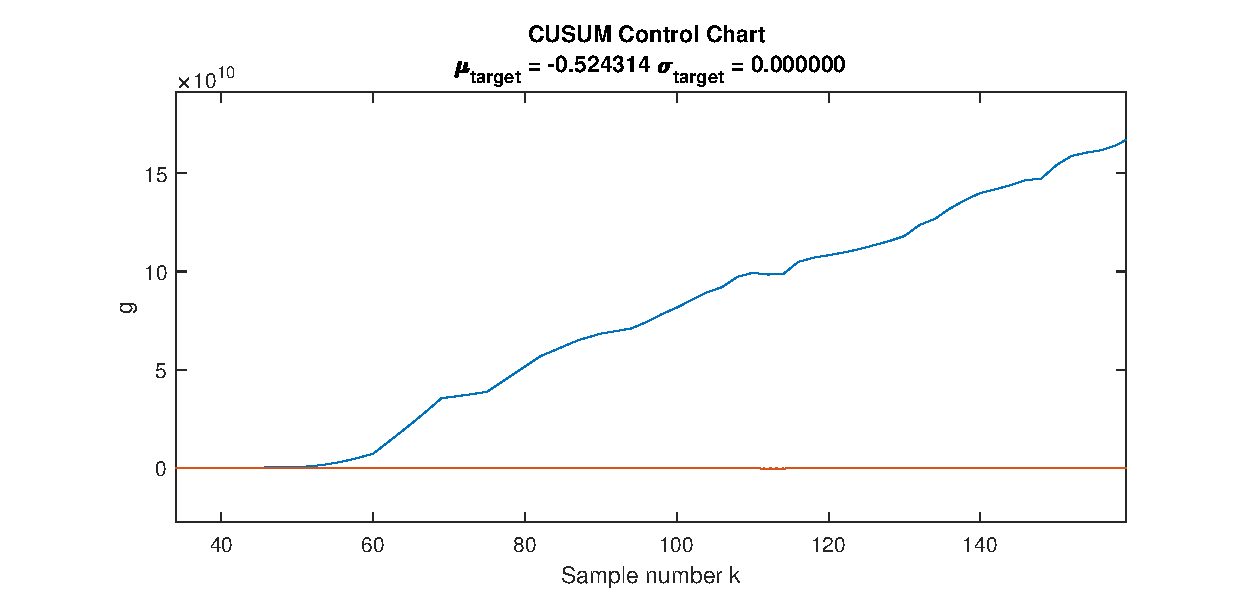
\includegraphics[width=0.7\linewidth]{figures/cusum1}
% 	\caption{CUSUM output with fault on the z axis magnetorquer at 40s }
%	\label{fig:cusum1}
%\end{figure}  


\subsection{Luenberger Observer} 
\label{sec:simpleObserver}

Parallel to structural analysis method an observer based method have been designed for fault detection in magnetorquer based actuators. Here will be discussed a Luenberger-like form which is based directly on the non-linear dynamics. In previous chapter has been discussed that for each axis there is a pair of magnetorquers. The redundant magnetic actuators are used for reconfiguration in the presence of a fault or failure.\\    The Luenberger-like observer is based on the dynamic equation \ref{eq:seom} and for the sake of brevity is rewritten here as   

%
\begin{flalign}
\vec{\dot \omega}	
= 
{-\underline{I}_{s}^{-1} \underline{\omega}^\times \underline{I}_{s}\vec{\omega}-\underline{I}_{s}^{-1}\underline{\omega}^\times \vec{h_{rw}}+\underline{I}_{s}^{-1}[\vec{N_{rw}} + \vec{N_{mt}}+\vec{N_{dist}}}]
\label{eq:seom22}
\end{flalign}
%
where the time dependency of the variables has been suppressed for clarity. Rearranging the above equation and by adding the fault vector $\vec{F_{MT}}$ it can obtained 
%
\begin{flalign}
\vec{\dot \omega}	
= 
\underbrace{-\underline{I}_{s}^{-1}  [(\underline{I}_{s}\vec{\omega})^\times- (\vec{h_{rw}})^\times]}_{\underline{A}}\vec{\omega}+\underbrace{\underline{I}_{s}^{-1}}_{\underline{B}} \underbrace{[\vec{N_{rw}} + \vec{N_{mt}}]}_{\vec{u}}+\underline{I}_{s}^{-1}\vec{N_{dist}}+\vec{{F}_{MT}}
\label{eq:seom2244}
\end{flalign}
%  
where $\underline{A}=-\underline{I}_{s}^{-1}  [(\underline{I}_{s}\vec{\omega})^\times- (\vec{h_{rw}})^\times] $ is the system matrix, $ \underline{B}= \underline{I}_{s}^{-1}$ is the input matrix, $\vec{N_{actual}} =\vec{N_{rw}} + \vec{N_{mt}} $ is the input vector and $\vec{N_{dist}}= \vec{d}$ is the disturbance vector. The system can now be written in Luenberger-like form as
%
\begin{flalign}
\vec{\dot{{\hat \omega}}} = \underline{A}{\hat{{\vec{\omega}}}}+\underline{B}\vec{u}+\underline{B}\vec{d}+\underline{L}\underline{C}({\vec{\omega}}-{\hat{{\vec{\omega}}}})
\label{eq:seom255554}
\end{flalign}
% 
with $\underline{L}$ be the observer gain and the output vector can be written as
\begin{flalign}
\vec{y} = \underline{C}\hat{\vec{\omega}}
\label{eq:seom2554}
\end{flalign}
with $\underline{C}$ be identity matrix. The matrix $\underline{A}$ is found by using the maximum values of $\vec{\omega}$ and $\vec{h_{rw}}$ which were obtained by running the simulation over one period, and thus the gain matrix is obtained by pole placement as
\begin{equation}
\underline{L}  = 
\begin{bmatrix}
-3.0000       & -0.0014 &  0.0004 \\
0.0011       &-4.0000  &  -0.0163  \\
-0.0003    &  0.0163   & -5.0000
\end{bmatrix} 
\label{eq:orthoMatrix22}
\end{equation}
%
\subsubsection{Residual generation}
 %
 Assuming that the motors are fault free a residual can be generated from the Luenberger-like observer. By denoting $\vec{N_{obs}} =\vec{I_s}\vec{\dot{{\hat \omega}}}$ where $I$ is the inertia of the satellite then a residual can be generated as
 
 %
 \begin{equation}
 residual = \vec{N_{actual}} - \vec{N_{obs}}
 \label{eq:residualObs}
 \end{equation}
 %
 thus if $\lVert \vec{residual} \rVert \geq threshold$ a fault has been occurred. The structure of Luenberger-like observer can be seen in \figref{fig:obe} and the generated residual signal in \figref{fig:observerresidual} . 
 %
 \begin{figure}[H]
 	\centering
 	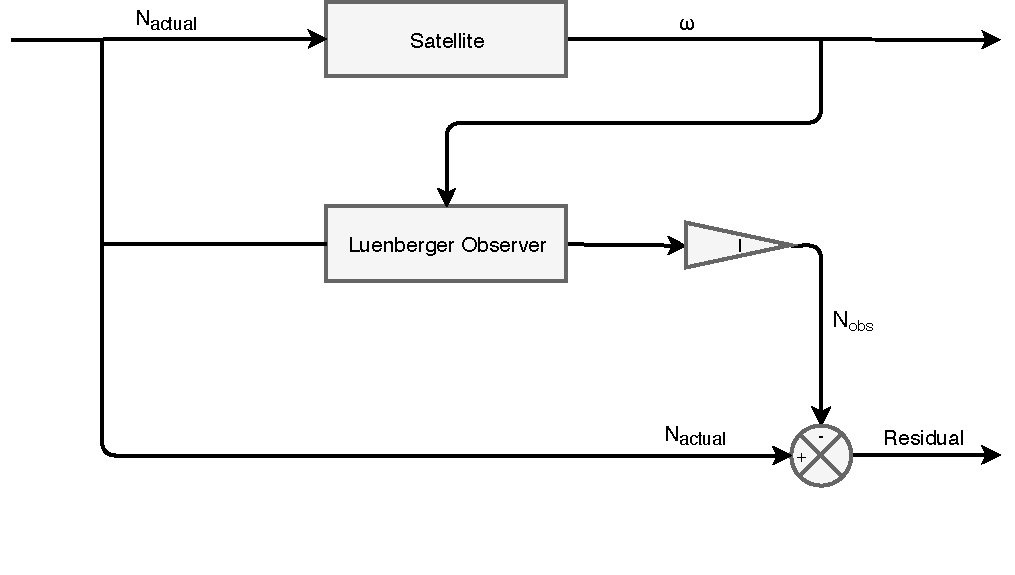
\includegraphics[width=0.7\linewidth]{figures/observerSimple}
 	\caption{Luenberger-like observer structure and residual generation}
 	\label{fig:obe}
 \end{figure}
 %
 \label{sec:simpleObserveresidual}
 %
\begin{figure}[H]
	\centering
	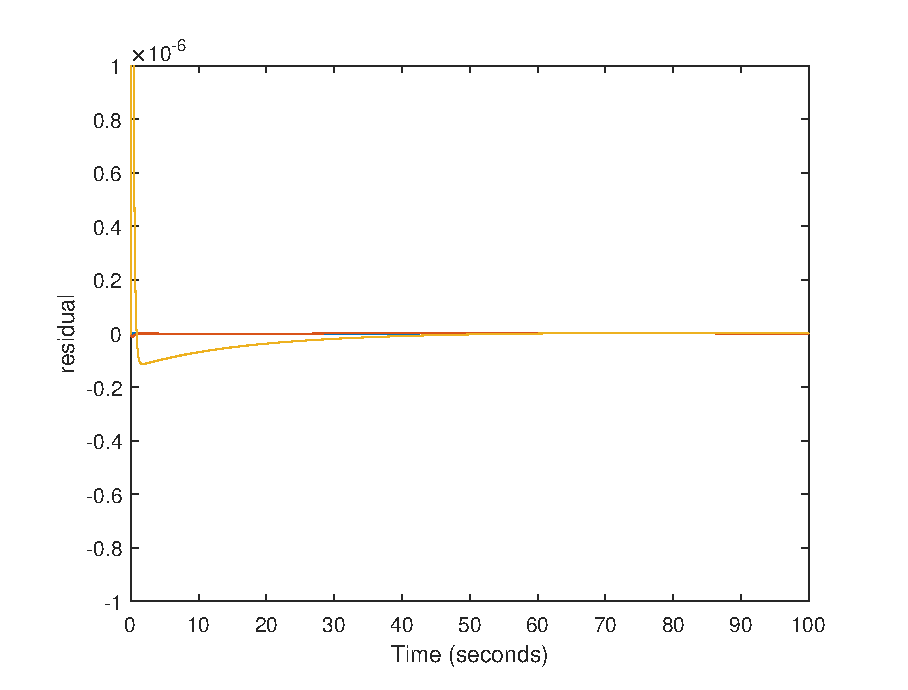
\includegraphics[width=0.7\linewidth]{figures/Observer_residual}
	\caption{Luenberger-like Observer residual signal }
	\label{fig:observerresidual}
\end{figure}
%
 Even the Luenberger-like observer is able to detect certain faults, is not robust in the sense of isolation. In order to isolate the faulty component the  Luenberger-like observer can be combined with the local structural analysis based residual which have been discussed in \ref{sec: MTStructAnal} and together by combining their flags can reconfigure the magnetorquer scheme by shutting off the faulty component and turning on the healthy one which will be discussed in chapter \ref{chap:faltHandling}. In the \figref{fig:obsflag} it can be seen the flag from the observer with a fault in the voltage supply of the first magnetorquer component at $200$[s]. 
 %
 \begin{figure}[H]
 	\centering
 	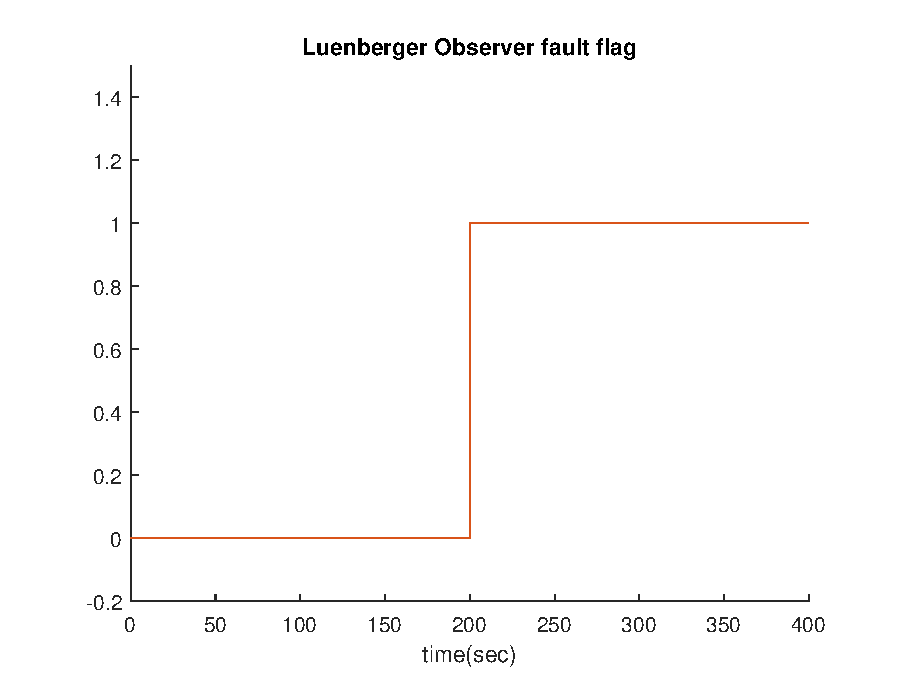
\includegraphics[width=0.7\linewidth]{figures/Luenberger_Observerflag}
 	\caption{Luenberger-like Observer flag with a fault in the voltage supply occurring at 200 seconds   }
 	\label{fig:obsflag}
 \end{figure}

%


\subsection{Unknown Input Observer (UIO)} \label{sec:UIO}
Disturbances and modeling errors may cause discrepancies between the actual system and the descriptor mathematical model. Linearization and simplifications which make the system more manageable may lead to such uncertainties. Uncertainties can have an effect on the system dynamic behavior. During observer design, these uncertainties can be considered as unknown inputs. The observer can be designed to make the system state estimate error converge to zero in the presence of such unknown inputs. The linearized system dynamics is described according to equations \ref{stateObs} and \ref{eq:ui2}.
  
  \todo{reference lecture notes}
%A residual, fault indicator, based on observer design can be robust regarding the unknown input signals by making the effect of unknown inputs (UI) insensitive to the residual and thus making possible to maximize the detectability of a fault. The dynamic equation of the system can be written as  

%\nomenclature[A]{\textbf{UI}}{Unknown Input}
%

\nomenclature[AU]{\textbf{UIO}}{Unknown Input Observer }

\begin{equation}
\dot{\vec{x}} = \underline A\vec{x}+\underline B \vec{u}+\underline E\vec{d}
\label{stateObs}
\end{equation}
\begin{equation}
\vec{y} = \underline C \vec{x}
\label{eq:ui2}
\end{equation}
%
where $\underline A$ ,$\underline B$ and $ \underline C $ are the system matrix, input and output matrix respectively and $\underline E$ is the distribution matrix of the unknown input (disturbance) $\vec{d}$. Furthermore, $\vec{x}$ is the state vector, $\vec{u}$ is the input vector and $\vec{y}$ is the output vector. The time dependency of the variables has been suppressed in order to relax the notation. Following \cite{UIO}, 
%
%
\\
\textit{An observer is defined as Unknown Input Observer for a system described by \eqref{stateObs} if the state estimation error vector $e$ approaches zero asymptotically regardless of the presence of the unknown input }
\\
The full order observer dynamics is set up according to equations \ref{stateObs1} and \ref{stateObs2}.
\begin{equation}
\dot{\vec{z}} = \underline F\vec{z}+\underline{TB} \vec{u}+\underline K\vec{y}
\label{stateObs1}
\end{equation}
\begin{equation}
\hat{\vec{x}} = \vec{z} + \underline H \vec{x}
\label{stateObs2}
\end{equation}

with $\hat{\vec{x}}$ being the state estimate and $\vec{z}$ the state of the observer. When \eqref{stateObs1} is an observer for the system given by \eqref{stateObs} the dynamics of the error  vector ($\vec{e} = \vec{x} - \hat{\vec{x}}$) can be written according to equation \ref{errordynamics} \cite{UIO}.
\begin{equation}
\dot{\vec{e}}= (\underline A-\underline H \underline C \underline A-\underline K1 \underline C)\vec{e} + (\underline A-\underline H \underline C \underline A-\underline K1 \underline C - \underline F)\vec{z}+ ((\underline A-\underline H \underline C \underline A-\underline K1 \underline C )\underline H-\underline K2)\vec{y}
\label{errordynamics}
\end{equation}
\begin{equation*}
+ (\underline I - \underline {HC} - \underline T)\underline B\vec{u}	+(\underline I -\underline H\underline C)\underline E \vec{d}
\label{errordynamics45}
\end{equation*}
in the above equation the utility of $\vec{x}  = \vec{e} + \hat{\vec{x}} = \vec{e} + \underline H\vec{y}+\vec{z}$ is used. The estimation error may converge to zero if the following conditions hold true:
%
\begin{equation}
\underline F = \underline A-\underline H \underline C \underline A-\underline K1 \underline C
\label{errordynamics3}
\end{equation}
\begin{equation}
(\underline I - \underline{HC})\underline E = 0
\label{errordynamics4}
\end{equation}
\begin{equation}
\underline T = (\underline I - \underline H\underline C)
\label{errordynamics5}
\end{equation}
\begin{equation}
\underline K = \underline K_{1} +\underline K_{2}
\label{errordynamics6}
\end{equation}
\begin{equation}
\underline K_{2} =\underline F \underline H 
\label{errordynamics7}
\end{equation}
where $\underline K_{1}$ is designed freely by pole placement to give desired eigenvalues of the observer. The error dynamics if equations \ref{errordynamics4}-\ref{errordynamics7} hold true can now be written as 
\begin{equation}
\dot{\vec{e}} = \underline F \vec{e}
\label{errordynamics8}
\end{equation}
consequently if the eigenvalues of $\underline F$ are to the left half plane, the error converges exponentially to zero. 

A solution to \eqref{errordynamics4} is given by making use of the Moore-Penrose pseudo-inverse as
\begin{equation}
\underline H = \underline E (\underline{CE})^\dagger
\label{errordynamics9}
\end{equation}
with $(\underline{CE})^{+} = [(\underline{CE})^{T} (\underline{CE})]^{-1}\underline{CE})^{T} $.
A sufficient and necessary condition for the UIO existence is that the number of independent unknown inputs can not be larger than the number of independent measurements which leads to
\begin{equation}
rank (\underline{CE}) =rank( \underline E) 
\label{errordynamics10}
\end{equation}
and by denoting $\underline A_1 = \underline A - \underline{HCA} $ that the pair $(\underline {CA}_1)$ is detectable and thus $F$ can have stable roots.


\subsubsection{Residual Generation}

In order to be able to detect faults, a residual signal is set up.  The residual should converge to zero in the presence of $\vec{d}$ unknown input and the absence of faults. In order to make the faults strong detectable, the residual should not converge to zero in the presence of faults. The residual is defined as
%The residual is used for fault detection and isolation thus should be decoupled from the unknown inputs(disturbances). The residual can be written as
\begin{equation*}
\vec{r} = \vec{y} - \underline C \hat{\vec{x}} 
\label{errordynamics11} = 
= \vec{y} - \underline C (\vec{z} + \underline{H} \vec{y} ) 
= (\underline I  -\underline{ CH})\vec{y}   -\underline C \vec{z} 
\end{equation*}

which does not depend on the disturbance vector. Residual thresholding can be applied to detect faults.
% A simple threshold can be applied such that for the faulty case, if the magnitude of the residual is larger than the threshold then a fault has been occurred as
%$\{\lVert \vec{r}\rVert \geq threshold \}$ else if $\{\lVert \vec{r}\rVert < threshold \}$ then the system is fault free.
Figure \ref{fig:residualobs} illustrates the nominal unknown input observer with a block diagram. 
%of the nominal system and the observer can be seen along with the residual generator
\begin{figure}[H]
	\centering
	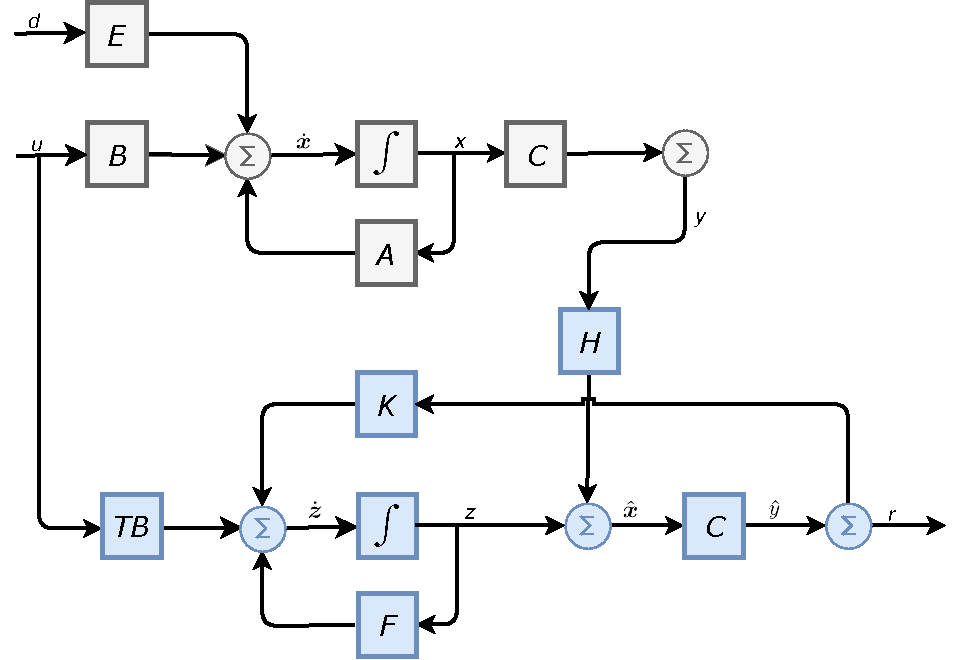
\includegraphics[width=0.8\linewidth]{figures/UIO}
	\caption{Observer based residual generator}
	\label{fig:residualobs}
\end{figure}

%Moreover, in figure \ref{fig:residualobstest} it can be seen how the state error converge asymptotically to zero from the initial conditions along with a change in the attitude of the satellite after 70 seconds.

%\begin{figure}[H]
%	\centering
%	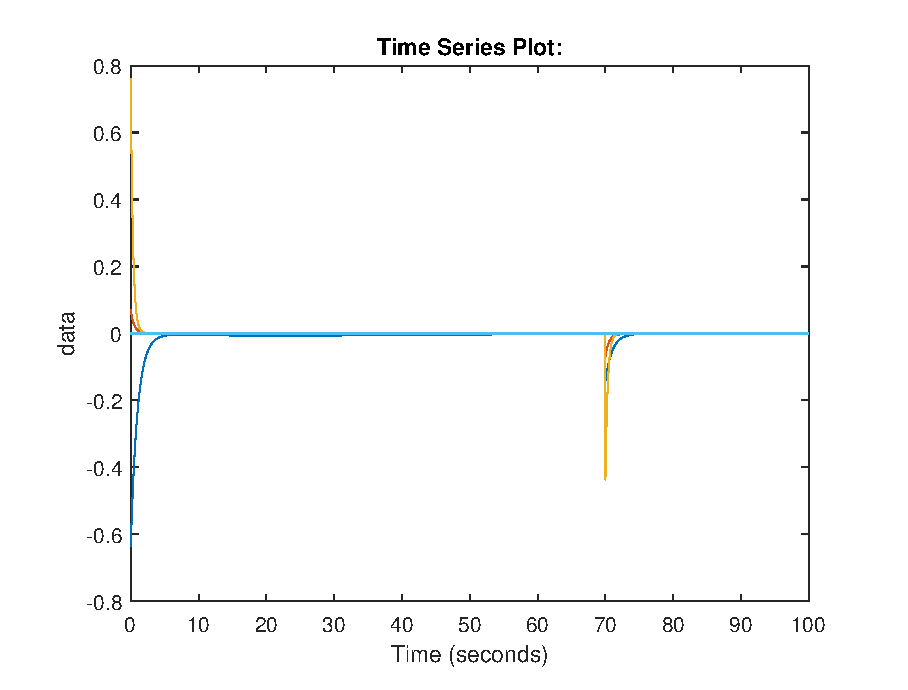
\includegraphics[width=0.7\linewidth]{figures/obstest}
%	\caption{Convergence of the state estimation error to zero with the disturbance been decoupled}
%	\label{fig:residualobstest}
%\end{figure}

Actuator fault isolation is possible assuming that all the sensors are fault free. Sensor fault isolation is possible assuming that the actuators are fault free. A descriptor model of the overall system with actuator fault can be written as given in equation \ref{stateObs}.
\begin{equation}
\dot{\vec{x}} = \underline A\vec{x}+\underline B \vec{u}+\underline E\vec{d} + \underline B\vec{f_{act}}
\label{stateObs34}
\end{equation}
where $\vec{f_{act}}$ represents the actuator faults. 

In order to isolate faults, separate UIOs need to be constructed for each actuator. The observer matrices are adjusted for each actuator by deleting the column of the matrix B corresponding to the actuator, namely $\vec{b_{i}}$ and incorporating this along with the disturbance distribution matrix as
\begin{equation*}
E^{i} = [ E  \vec{b_{i}}]
\label{errordynamics14}
\end{equation*}
and furthermore, the $i_{th}$ component of the input vector $u_{i}$ is incorporated to the disturbance vector as 
\begin{flalign*}
\begin{bmatrix}
\vec{d} \\ u_{i}+f^{i}_{act}
\end{bmatrix}
\end{flalign*} 
leading to a bank of observers with each residual actuated by 2 inputs(without $i_{th}$) and all outputs. The detection of the fault is made by applying a threshold as  $\{\lVert r^{i}\rVert < Thr^{i} \}$ else if $\{\lVert r^{k}\rVert \geq Thr^{k} \}$ with $k = 1,...i-1,..i+1,5..r$.

\todo{is the last paragraph ok?}

%\subsection{CUSUM algorithm and change detection} 
%The evaluation of the residual which determines if the %actuator is faulty or fault free is based on the %cumulative sum (CUSUM), a sequential hypothesis %testing technique to detect changes on the noisy %signal. By changes are accounted changes on the mean %of the original signal. 



% \begin{figure}[H]
%	\centering
% 	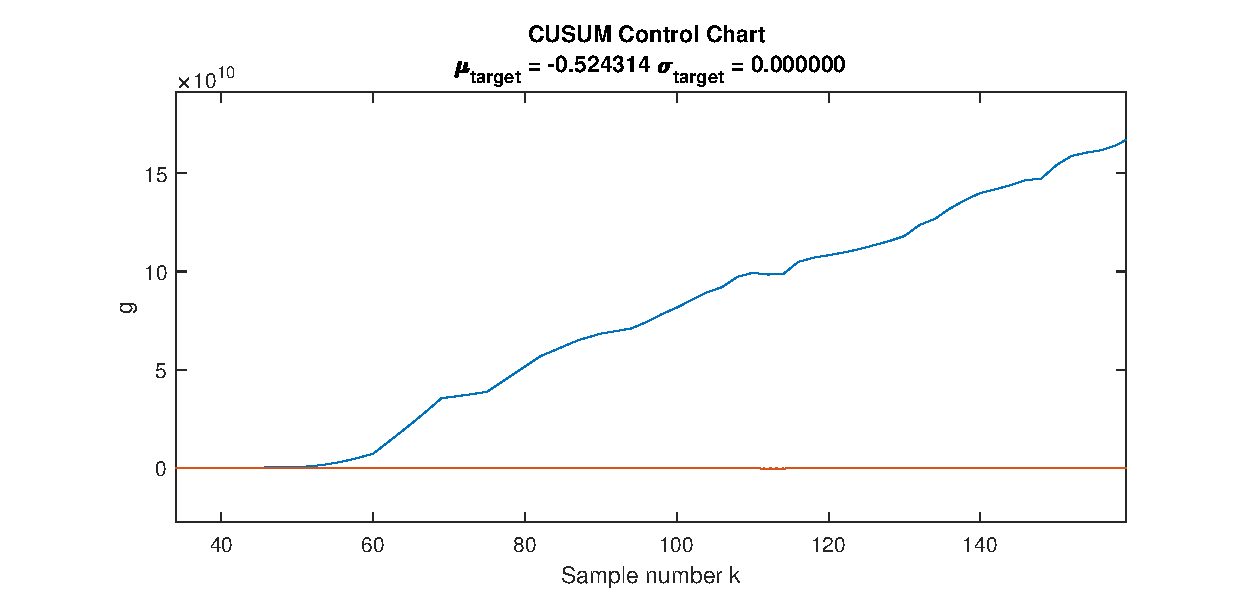
\includegraphics[width=0.7\linewidth]{figures/cusum1}
% 	\caption{CUSUM output with fault on the z axis magnetorquer at 40s }
%	\label{fig:cusum1}
%\end{figure}  



\subsection{Application of Unknown Input Observer}
\label{sec:UIO_App}

\todo{discuss articles a bit}

The present chapter discusses how to apply unknown input observer (UIO) theory to the satellite functioning in nadir pointing control goal. The regular UIO uses linear model, however the satellite system is highly nonlinear.  During one orbit, the orientation of the nadir pointing satellite rotates by $360\deg$. By choosing the appropriate reference frame, this rotation can be eliminated from attitude dynamics. In local vertical, local horizontal frame (LVLH), the nadir pointing satellite keeps its attitude. This opens an opportunity to use linear approximation of the trigonometric nonlinearities in the satellite dynamic equations. The operating point should be chosen as nadir pointing, and if the attitude stays near enough to the operating point, the model stays quite accurate.

\todo{add LVLH to frames chapter}

Yang's article on desaturation \cite{DesatYang} describes a model that can be effective for UIO. The $\underline{A}$ matrix of the model is constant, so the UIO matrices can be derived as described in \ref{sec:UIO}. The model detaches the orbit angular velocity from the dynamics according to equation \ref{eq:angDetach}.

\begin{equation}
\label{eq:angDetach}
\vec{\omega} = \vec{_I^{lv}\omega} + \vec{_{lv}^s\omega}
\end{equation}

where $\vec{_I^{lv}\omega}$ is the angular velocity of the LVLH frame compared to the inertial frame and $\vec{_{lv}^s\omega}$ is the angular velocity of the body frame compared to the LVLH frame.

\todo{should we show the equations in more detail?}

\begin{equation}
\vec{\dot{x}} =
\underline{A}\vec{x} + \underline{B}(t)\vec{u} + \underline{E} \vec{d} + \underline{F}_x \vec{f} 
\end{equation}

\tiny
\begin{align}
\begin{bmatrix}
\vec{_{lv}^s\dot{\omega}} \\
\vec{\dot{\omega}_{rw} } \\
\vec{\dot{q}_{1:3}}
\end{bmatrix} 
 \nonumber
= \begin{bmatrix}
0 & 0 & \omega_o\frac{I_1 - I_2 + I_3}{-I_1} & 0 & 0 & \omega_o\frac{I_w}{-I_1} & 8\omega_o^2\frac{I_3 - I_2}{I_1} & 0 & 0 \\
0 & 0 &	0 & 0 & 0 &	0 & 0 &  6\omega_o^2\frac{I_3 - I_1}{I_2} & 0\\
 \omega_o\frac{I_1 - I_2 + I_3}{I_3}  & 0 & 0 &  \omega_o\frac{I_w}{I_3} & 0 &	0 & 0 & 0 & 2\omega_o^2\frac{I_1 - I_2}{I_3}\\
0 & 0 &	0  & 0 & 0 & 0 & 0 & 0 & 0\\
0 & 0 &	0  & 0 & 0 & 0 & 0 & 0 & 0 \\
0 & 0 &	0 & 0 & 0 & 0 & 0 & 0 & 0\\
0.5 & 0 &	0 & 0 & 0 & 0 & 0 & 0 & 0 \\
0 & 0.5 &	0& 0 & 0 & 0 & 0 & 0 & 0 \\
0 & 0 &	0.5 & 0 & 0 & 0 & 0 & 0 & 0\\
\end{bmatrix}
\begin{bmatrix}
_{lv}^s\omega_1 \\
_{lv}^s\omega_2 \\
_{lv}^s\omega_3 \\
\omega_{rw,1} \\
\omega_{rw,2} \\
\omega_{rw,3} \\
q_1 \\
q_2 \\
q_3 
\end{bmatrix}
 \\
 \nonumber
+
\begin{bmatrix}
I_1^{-1} & 0 & 0 & 0 & \frac{b_3}{I_1} & -\frac{b_2}{I_1}	& I_1^{-1} & 0 & 0\\
0 & I_2^{-1} & 0 & - \frac{b_3}{I_2} & 0 &  \frac{b_1}{I_2} & 0 & I_2^{-1} & 0\\ 
0 & 0 & I_3^{-1} &  \frac{b_2}{I_3} &  -\frac{b_1}{I_3} & 0 & 0 & 0 & I_3^{-1} \\  
I_w^{-1} & 0 & 0 & 0 & 0 & 0 & 0 & 0 & 0 \\
0 & I_w^{-1} & 0 & 0 & 0 & 0 & 0 & 0 & 0 \\ 
0 & 0 & I_w^{-1} & 0 & 0 & 0 & 0 & 0 & 0\\  
0 & 0 & 0 & 0 & 0 & 0 & 0 & 0 & 0\\
0 & 0 & 0 & 0 & 0 & 0 & 0 & 0 & 0\\
0 & 0 & 0 & 0 & 0 & 0 & 0 & 0 & 0\\
\end{bmatrix}
\begin{bmatrix}
N_{rw,1} \\
N_{rw,2} \\
N_{rw,3}\\
\m_{mt,1} \\
\m_{mt,2} \\
\m_{mt,3} \\
N^{est}_{dist,1} \\
N^{est}_{dist,2} \\
N^{est}_{dist,3}
\end{bmatrix}
+
\begin{bmatrix}
I_1^{-1} & 0 & 0 \\
0 & I_2^{-1} & 0 \\
0 & 0 & I_3^{-1}\\
0 & 0 & 0 \\
0 & 0 & 0 \\
0 & 0 & 0 \\
0 & 0 & 0 \\
0 & 0 & 0 \\
0 & 0 & 0 
\end{bmatrix}
\begin{bmatrix}
N^{est \ error}_{dist,1} \\
N^{est \ error}_{dist,2} \\
N^{est \ error}_{dist,3}\\
\end{bmatrix}
 \\
 + 
 \begin{bmatrix}
 I_1^{-1} & 0 & 0 & 0 & \frac{b_3}{I_1} & -\frac{b_2}{I_1}\\
 0 & I_2^{-1} & 0 & - \frac{b_3}{I_2} & 0 &  \frac{b_1}{I_2} \\ 
 0 & 0 & I_3^{-1} &  \frac{b_2}{I_3} &  -\frac{b_1}{I_3} & 0 \\  
 I_w^{-1} & 0 & 0 & 0 & 0 & 0 \\
 0 & I_w^{-1} & 0 & 0 & 0 & 0 \\ 
 0 & 0 & I_w^{-1} & 0 & 0 & 0 \\  
 0 & 0 & 0 & 0 & 0 & 0 \\
 0 & 0 & 0 & 0 & 0 & 0 \\
 0 & 0 & 0 & 0 & 0 & 0 \\
 \end{bmatrix}
 \begin{bmatrix}
 N^{fault}_{rw,1} \\
 N^{fault}_{rw,2} \\
 N^{fault}_{rw,3}\\
 \m^{fault}_{mt,1} \\
 \m^{fault}_{mt,2} \\
 \m^{fault}_{mt,3} 
 \end{bmatrix}
\label{eq:uioMatrices}
\end{align}
\normalsize

where $I_w$ is the reaction wheel axial moment of inertia, $\omega_o$ is the angular velocity of the orbit, $I_i$ is the satellite moment of inertia along $i$th principal axis.

\nomenclature[SIw]{$I_w$}{Reaction wheel axial moment of inertia}

\nomenclature[Somegao]{$\omega_o$}{Orbit angular velocity}

\begin{figure}[H]
	\centering
	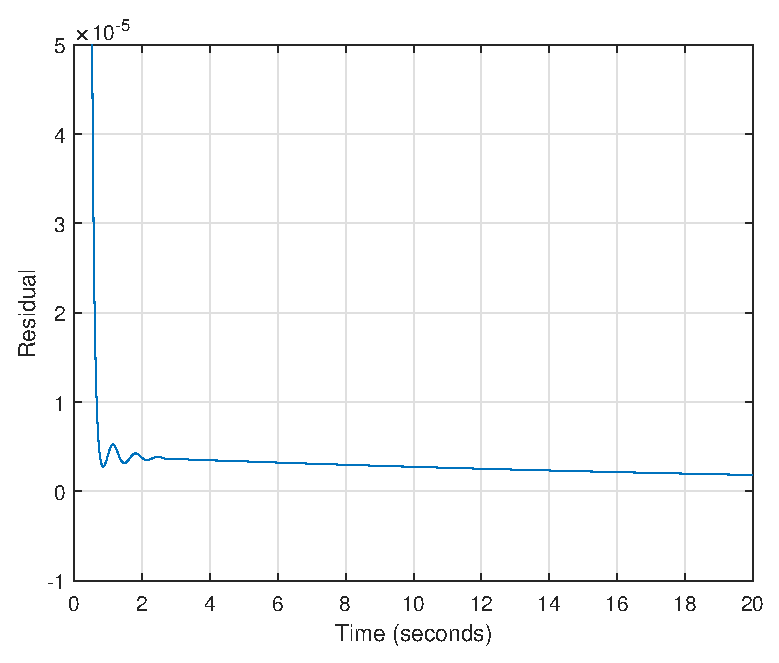
\includegraphics[width=0.7\linewidth]{figures/nosensfault_res}
	\caption{no sensor fault }
	\label{fig:}
\end{figure}

\begin{figure}[H]
	\centering
	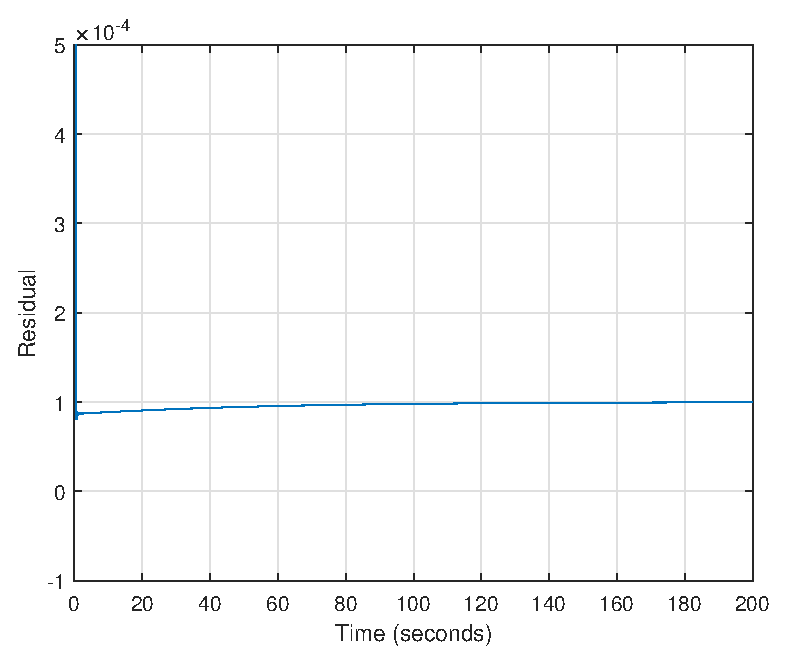
\includegraphics[width=0.7\linewidth]{figures/sensfault_res}
	\caption{sensor fault 0.1 ang vel x excess}
	\label{fig:}
\end{figure}

\begin{figure}[H]
	\centering
	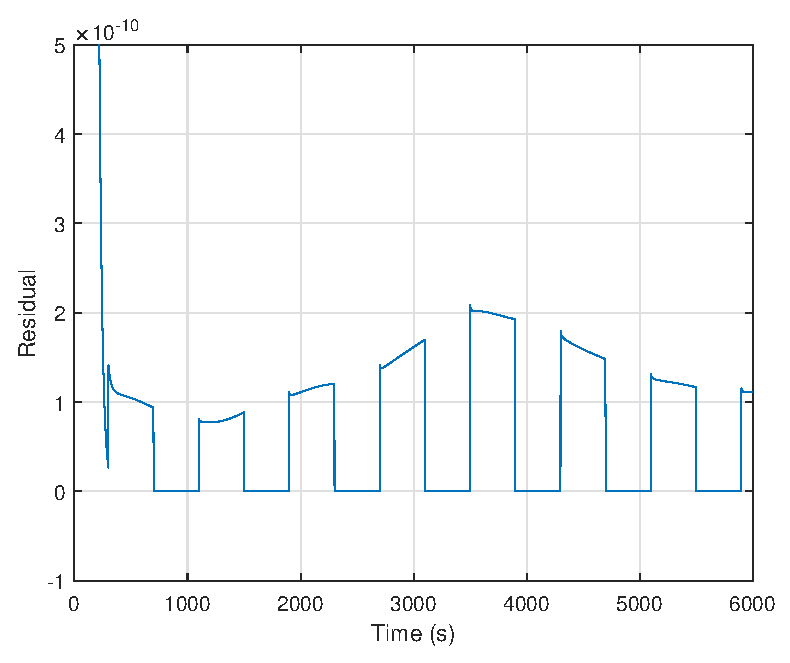
\includegraphics[width=0.7\linewidth]{figures/mt_fault_res}
	\caption{mmt error}
	\label{fig:residualmt}
\end{figure}

\begin{figure}[H]
	\centering
	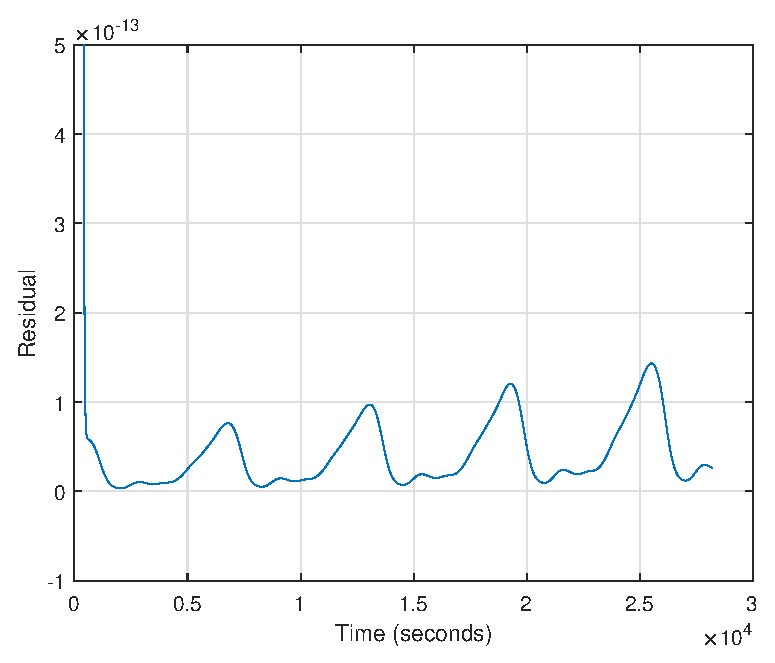
\includegraphics[width=0.7\linewidth]{figures/constdistonly_res}
	\caption{only dist const}
	\label{fig:residualdist}
\end{figure}

\begin{figure}[H]
	\centering
	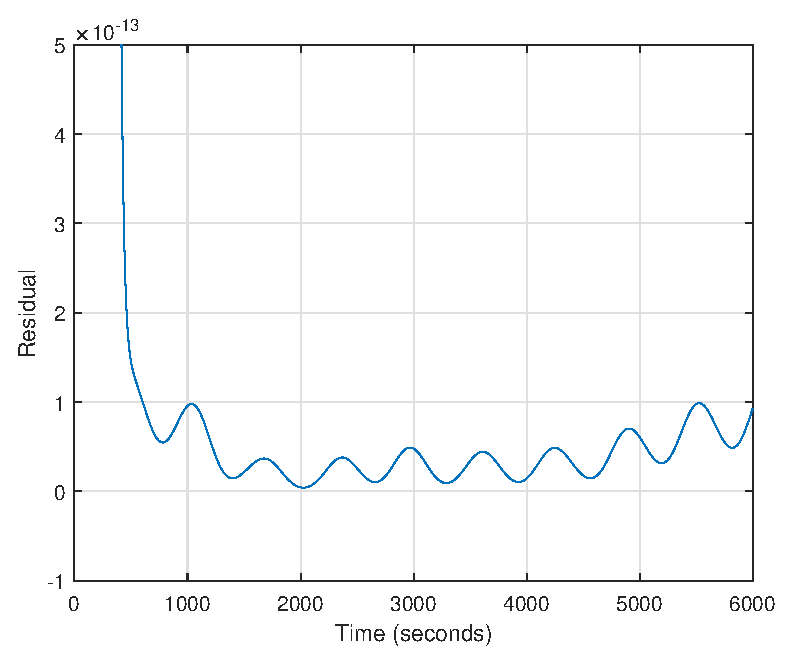
\includegraphics[width=0.7\linewidth]{figures/distonly_res}
	\caption{only dist sine}
	\label{fig:}
\end{figure}

%\nomenclature[Sw]{$\omega_o$}{Orbit angular velocity}


\subsection{Virtual actuators and sensors} \label{chap: virtual}
Actuators and sensors are subject to various faults in the process. Due to these faults the system may experience drops in the performance which could lead to stability loss.

The objective of fault tolerant control using virtual actuators and sensors is to add a reconfiguration block which is presented as an extra layer between the faulty system and the controller, while the nominal controller is running. The purpose of the reconfiguration block in case of a fault is to provide fault tolerance by using the virtual actuators and sensors as can be seen in figure \ref{fig:VA}.

\begin{figure}[H]
	\centering
	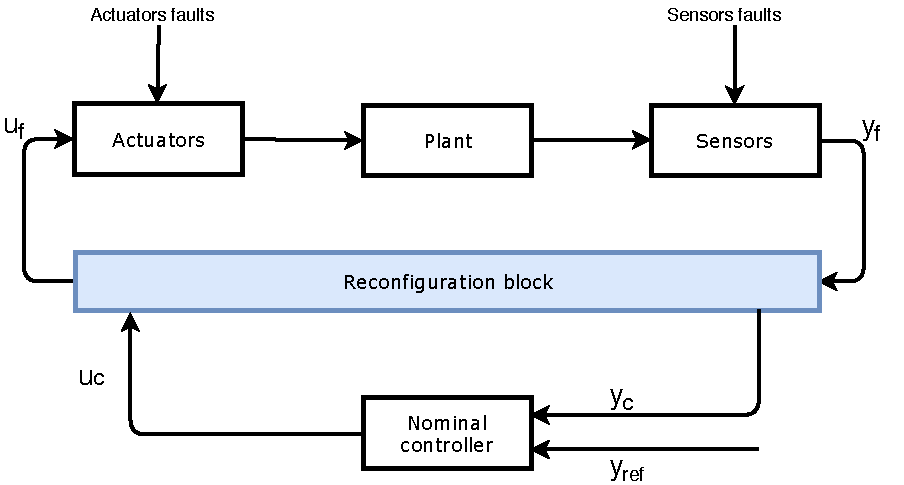
\includegraphics[width=0.8\linewidth]{figures/VirtualActuator}
	\caption{ Virtual actuators and sensors scheme}
	\label{fig:VA}
\end{figure}

If that the main controller remain unchanged, a reconfiguration between the system and the output of the controller is made. If a fault in the actuators or sensors will occur, then the reconfiguration block has the possibility to give as an output a signal that is similar with the one that the actuator or sensor will have for the nominal controller.

In the case that a fault will occur in the reaction wheel sensor, the angular velocity measurement it is assumed functional and based on that measurement, the torque output form the faulty wheel can be computed. A second assumption is that the sensors will completely fail, but in this case a model of how the angular velocity of the wheel is decreasing over time is obtained. This model can be used as a virtual sensor for the angular velocity sensor. 


\subsection{Magnetorquers structural analysis} \label{chap: MTStructAnal}
For magnetorquers fault detection, two types of structural analysis were implemented. First, a locally structure analysis for each magnetorquer was implemented, and second a second a structure analysis using the satellite dynamics.

The residual for the magnetorquer is generated using the following equation:
\begin{flalign}
	residual = B - \frac{4 \mu_0}{\sqrt{2} \pi L} I
	\label{eq:BfS}
\end{flalign} 
where \\
$\vec B$ is the magnetic field \\
$\mu_0$ is a constant called permeability of free space \\
$I$ is the current \\
$L$ is the length of the coil

In equation \ref{eq:BfS} the magnetic field is measured and based on this measurement the magnetic moment can be deducted, but for the residual is not necessary, because if it is correct then the magnetic moment should be as expected using magnetic sensors for checking, unless the shape of the coil changes, perhaps due to some physical movement of the system.









